% --------------------------------------------------------------------------------

\begin{exercise}

Geben Sie, für jedes gerade $n \in \N$ paarweise unterschiedliche Schlüssel $x_1, \dots, x_n$ an, so dass ein Suchbaum in Kammform (sh. Abbildung) entsteht wenn, beginnend mit dem leeren Suchbaum, die Schlüssel $x_1, \dots, x_n$ in dieser Reihenfolge eingefügt werden.

\end{exercise}

% --------------------------------------------------------------------------------

\begin{solution}

\phantom{}

\includegraphicsboxed{DGA/DGA - Definition 5.1.png}
\includegraphicsboxed{DGA/DGA - Algorithmus 14 - Einfügen in einen Suchbaum.png}

\begin{center}
  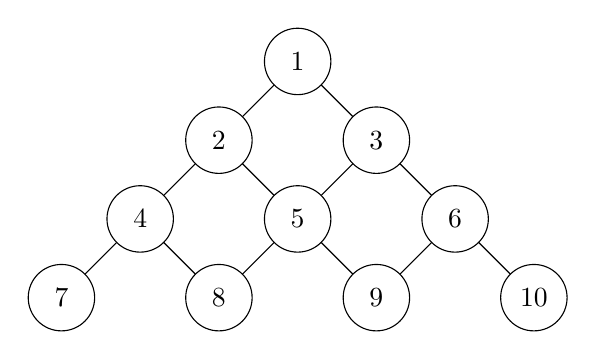
\begin{tikzpicture}

    \coordinate (x_1) at ( 0,  0);
    \coordinate (x_2) at (-1, -1);
    \coordinate (x_3) at ( 1, -1);
    \coordinate (x_4) at ( -2, -2);
    \coordinate (x_5) at ( 0, -2);
    \coordinate (x_6) at ( 2, -2);
    \coordinate (x_7) at (-3, -3);
    \coordinate (x_8) at (-1, -3);
    \coordinate (x_9) at (1, -3);
    \coordinate (x_10) at (3, -3);

    \draw (x_1) -- (x_2) -- (x_4) -- (x_7);
    \draw (x_1) -- (x_3) -- (x_6) -- (x_10);
    \draw (x_2) -- (x_5) -- (x_9);
    \draw (x_3) -- (x_5) -- (x_8);
    \draw (x_4) -- (x_8);
    \draw (x_6) -- (x_9);

    \filldraw [color = black, fill = white] (x_1) circle (12 pt) node {$1$};
    \filldraw [color = black, fill = white] (x_2) circle (12 pt) node {$2$};
    \filldraw [color = black, fill = white] (x_3) circle (12 pt) node {$3$};
    \filldraw [color = black, fill = white] (x_4) circle (12 pt) node {$4$};
    \filldraw [color = black, fill = white] (x_5) circle (12 pt) node {$5$};
    \filldraw [color = black, fill = white] (x_6) circle (12 pt) node {$6$};
    \filldraw [color = black, fill = white] (x_7) circle (12 pt) node {$7$};
    \filldraw [color = black, fill = white] (x_8) circle (12 pt) node {$8$};
    \filldraw [color = black, fill = white] (x_9) circle (12 pt) node {$9$};
    \filldraw [color = black, fill = white] (x_10) circle (12 pt) node {$10$};

\end{tikzpicture}

\end{center}

\begin{align*}
  x_i
  :=
  \begin{cases}
  i - 1, & \text{falls}~ i \in 2\N, \\
  i + 1, & \text{falls}~ i \in 2\N + 1,
  \end{cases}
  \quad
  i = 1, \dots, n
\end{align*}

\end{solution}

% --------------------------------------------------------------------------------
